
\section{Introducci�n}

\subsection{Definici�n del Problema}
\begin{frame}{Definici�n del Problema}

\framesubtitle{Reconocimiento de Actividades Humanas}
\begin{overprint}
\onslide<1> 
\begin{quote}
Determinar las acciones o comportamientos de uno o m�s individuos
a partir de datos ambiguos capturados por sensores situados en el
entorno.
\end{quote}
\onslide<2> 
\begin{block}<2>{Nota}
\emph{}El problema es conocido por sus siglas \structure{HAR} en
ingl�s \emph{(Human Activity Recognition})
\end{block}
\end{overprint}
\begin{center}
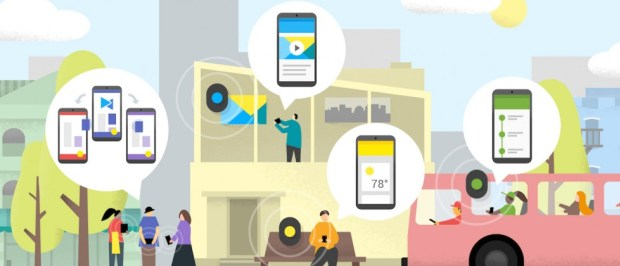
\includegraphics[width=0.8\textwidth]{intro/graphics/sensor-environment}
\par\end{center}

\end{frame}
%
\begin{frame}{Definici�n del Problema}

\setbeamercovered{transparent}

\framesubtitle{�Que es HAR?}
\begin{itemize}[<+->]
\item Es un t�pico de investigaci�n multidisciplinario que busca dise�ar
algoritmos para:
\begin{itemize}
\item Capturar movimientos de uno o m�s individuos en interacci�n con su
entorno 
\item Realizar aprendizaje e inferencia
\item Proveer informaci�n de contexto 
\end{itemize}
\end{itemize}
\begin{overprint}
\onslide<2> 
\begin{center}
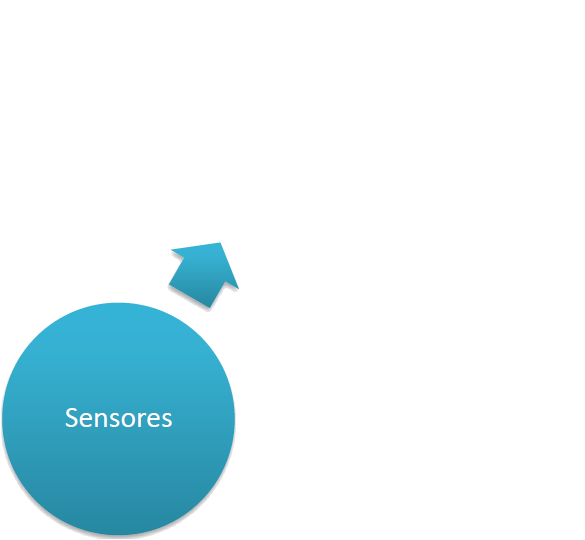
\includegraphics[width=4.5cm]{intro/graphics/areas-1}
\par\end{center}
\onslide<3> 
\begin{center}
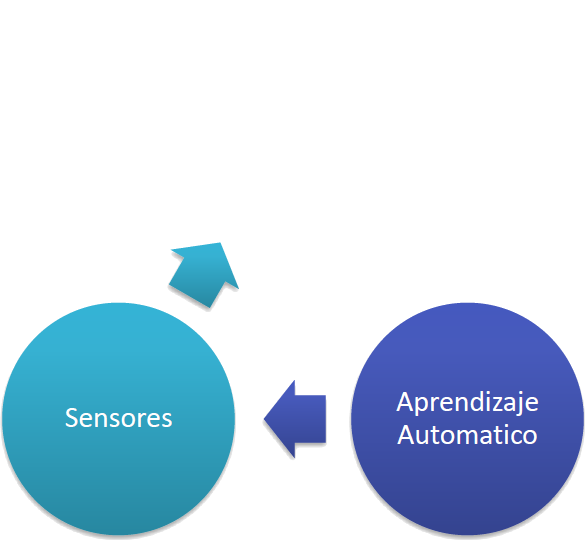
\includegraphics[width=4.5cm]{intro/graphics/areas-2}
\par\end{center}
\onslide<4> 
\begin{center}
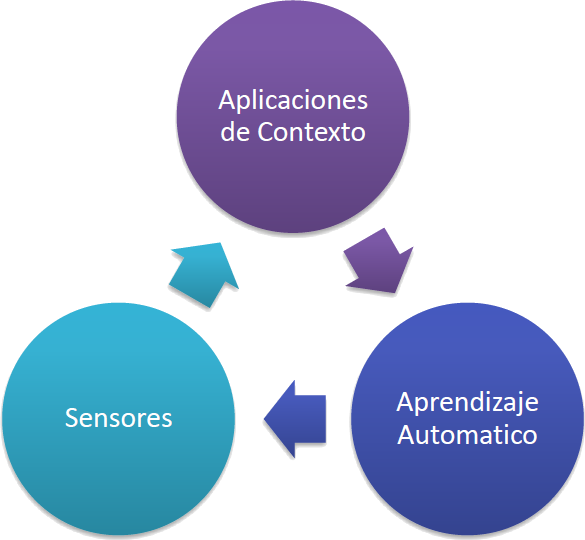
\includegraphics[width=4.5cm]{intro/graphics/areas-3}
\par\end{center}

\end{overprint}
\end{frame}
%
\begin{frame}{Definici�n del Problema}

\framesubtitle{Motivaci�n\setlength\columnsep{0pt}}
\begin{columns}

\column{0.5\textwidth}
\begin{itemize}[<+->]
\item El \structure{contexto} es primordial para los sistemas inteligentes 
\item Avances en tecnolog�as de \structure{computaci�n m�vil} y \structure{sensores} 
\item Uso intensivo de \structure{tel�fonos m�viles modernos} en la vida
diaria.
\item \setbeamercovered{transparent}Popularidad de \structure{aplicaciones m�viles}
de contexto en 
\begin{itemize}
\item el cuidado personal, 
\item la movilidad y 
\item la asistencia en la vida diaria 
\end{itemize}
\end{itemize}

\column{0.5\textwidth}
\begin{overprint}
\onslide<1> 
\begin{center}

\includegraphics[width=1\textwidth]{intro/graphics/context1}
\par\end{center}
\onslide<2> 
\begin{center}
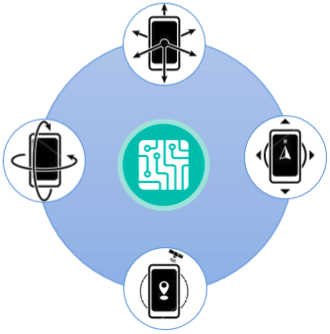
\includegraphics[width=1\textwidth]{intro/graphics/sensors}
\par\end{center}
\onslide<3> 

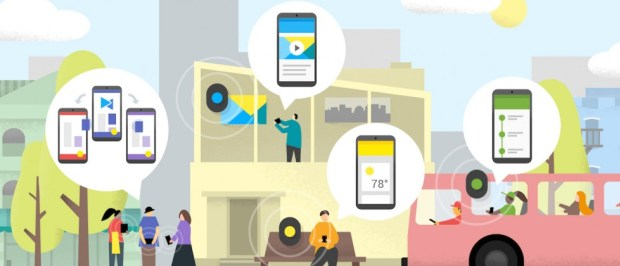
\includegraphics[bb=100bp 0bp 520bp 266bp,clip,width=1\textwidth]{intro/graphics/sensor-environment}
\onslide<4-> 


\includegraphics[width=1\textwidth]{intro/graphics/mobile-phone}
\end{overprint}
\end{columns}

\end{frame}
%
\begin{frame}{Definici�n del Problema}

\framesubtitle{Definici�n Teorica}

\begin{definition}[Problema HAR relajado]Dado (1) un conjunto $W=\{w_{0},...,w_{m-1}\}$
de $m$ ventanas de tiempo del mismo tama�o, donde cada una est� total
o parcialmente etiquetada, y que cada $w_{j}$ contiene un conjunto
de series de tiempo $S_{j}=\{s_{j,0},...,s_{j,k-1}\}$ para cada $k$
atributos medidos, y (2) un conjunto $A\text{=}\{\mathrm{a}_{0},...,\mathrm{a}_{n-1}\}$
de etiquetas de actividades, el objetivo es encontrar una funci�n
$f\colon S_{j}\rightarrow A$ que sea evaluada para todos los valores
posibles de $S_{j}$, tal que $f(S_{j})$ es lo m�s pr�ximo a la acci�n
realizada durante $w_{j}$ \end{definition}
\end{frame}

